\section{Experiments}
\label{sec:experiments}
We start by describing the datasets and workloads used before presenting the experimental results. 

\subsection{Experimental set-up}
\provalg\ was implemented in Java 8 using PostgreSQL 9.6.3 as the underlying DBMS. All experiments were conducted
on a Linux server \eat{Distribution? (Gianmaria)}with an Intel(R) Xeon(R) CPU E5-2630 v4 @ 2.20GHz and 64GB of main memory. 
Although there are provenance tools which support aggregate queries for relational database systems, e.g. GProM \cite{arab2018gprom}, they are overly complex for our purposes, and become a bottleneck for interactive computation. We therefore implemented a provenance layer from scratch, which simply collects how-provenance \cite{green2007provenance, amsterdamer2011provenance} for each query tuple.

\eat{
{\bf Provenance.} Provenance tools which support aggregate queries exist for relational systems, e.g. GProM \cite{arab2018gprom}. 
\eat{In GProM, each query tuple is associated with a set of tensors, which consists of how-provenance and aggregate values~\cite{amsterdamer2011provenance}. However, the aggregate values are not necessary for our purposes and become a bottleneck for interactive computation.}
However, they are overly complex for our purposes, and become a bottleneck for interactive computation. We therefore implemented a provenance layer from the scratch, which simply collects how-provenance for each query tuple.
}

{\bf Datasets.} %Three datasets were used in the experiments.
Two realistic datasets were used in addition to GENCODE: 
Hetionet\footnote{\url{https://neo4j.het.io/browser/}} and DBLP-NSF\footnote{\url{https://data.mendeley.com/datasets/ycnngyv5bd}}\cite{nsf_dblp}. 
Summary information about the three datasets, including the number of relations, average size per relation, and the size of the largest relation is presented in Table \ref{Table: datasets_summary}.

We converted Hetionet, which is stored in Neo4j, into a relational database\footnote{Available at 
\url{https://github.com/thuwuyinjun/Data_citation_provenance/files/2417454/hetionet_postgresql.zip}}.
% \scream{Should also make relational representation of Hetionet available.}
% Hetionet aims at building network to systematically identify why drugs work and predict new therapies for drugs. It connects some previously isolated information such as genes, drugs as well as biological processes in which drugs and genes may involve.
DBLP-NSF integrates DBLP publication information with NSF award information to augment traditional paper citations with funding information, and was developed in \cite{wu2018data}.

{\bf Workloads.} 
We test the performance of \provalg\ using both {\em synthetic} and {\em realistic} workloads. 
As mentioned earlier, to retrieve the provenance of aggregate views we can use either the {\em eager} or {\em lazy} strategy; we can also build an {\em index} on query provenance. We measure the performance gains using the {eager strategy} and index separately under both workloads. The performance also depends on the {\em policies}
used; different policies can lead to different results, and can generate either all or some of the covering sets. Due to space, only the case where {\em all} the covering sets are generated is presented here.

%only care about t_cs
The purpose of using {\em synthetic workloads} is to determine the key factors which influence performance. 
Extensive experiments were performed in~\cite{wu2018data} measuring the \textit{total reasoning time}  to generate the covering sets ($t_{cs}$) and the \textit{citation generation time}   after covering sets are constructed.  The \textit{citation generation time} is not considered here since \provalg\ only changes how {\em valid view mappings} are determined during covering sets construction process %(rather than {\em formatted citations}) 
relative to the implementations of \rba. Since \provalg\ relies on the query provenance for reasoning, the query time over the provenance-enabled database ($t_{q}$) is also recorded. The total execution time $t_{total}$ is measured as well, which is $t_q+t_{cs}$.
% in~\cite{wu2018data}.


%what key factors can influence the performance
%In terms of $t_{cs}$, based on the experimental results reported in \cite{wu2018data}, 
\eat{Maybe put in a table with these abbreviations in case people forget?}
In \cite{wu2018data}, $t_{cs}$ primarily depends on: 1) the number of view mappings (denoted $N_v$); 2) the total number of predicates under the view mappings (denoted $N_p$); and 3) the size of the query instance before duplicates are removed (which is the same as the total number of how-provenance monomials in the query instance $N_{pq}$). The experiments measure the effect of these metrics on $t_{cs}$. %Plus, according to the brief time complexity analysis in Section \ref{Sec: implementation}, 
The total number of how-provenance monomials in the view instance on average ($N_{pv}$) can influence performance according to the analysis in Section \ref{Sec: implementation}, and its effect is also considered in the experiments. So for the experiments for {\em synthetic workloads}, a query generator is built, which can generate random aggregate queries over GENECODE with $N_{pq}$ how-provenance monomials in total. Given a query $Q$ from this query generator, a view generator can generate $N_v$ views, each of which has $N_{pv}$ provenance monomials in total and has exact one view mapping to $Q$. 

%compare to TLA/SSLA
The trade-offs between \provalg\ and two implementations of  \rba\ proposed in \cite{wu2018data}, TLA and SSLA, are also  measured. 
% We do not consider the {\em pure view-based approach} of \cite{wu2018data},\scream{maybe not correct} since this does not generate fine-grained citations. %;  it is not difficult to extend the view-based approach to handle aggregate queries using conjunctive views. 
As mentioned before, \rba\ can be extended to handle aggregate queries when views are conjunctive views (but not aggregate views). In this case, TLA, SSLA and \provalg\ all generate the same final, fine-grained citations.
%, which derives us to conduct experiments in this setting.

% Plus, according to the complexity analysis in Section \ref{Sec: implementation}, the time to generate covering sets ($t_{cs}$) should also depend on the total number of how-provenance monomials in query and view instance (denoted $N_{pq}$ and $N_{pv}$ respectively) when the views are aggregate views while queries are aggregate queries, which is also experimentally verified herein.

In the {\em realistic workloads}, we use frequent queries against the three databases, and build views to represent the portions of data in the database associated with predefined citations. Both the synthetic and realistic views and queries used are available in our Github repository\footnote{\url{https://github.com/thuwuyinjun/Data_citation_provenance}}. 

To represent the summary information provided by GENCODE, we defined aggregate views to compute the total number of transcripts per gene, and the total number of exons per gene and per transcript. Two additional parameterized views are also defined to represent basic information (e.g. ID, name and type) for each transcript and gene, respectively. The realistic queries  compute the total number of exons ($q1$) and the total number of transcripts per type of gene ($q2$) respectively.

For DBLP-NSF we use the realistic views defined in \cite{wu2018data}. We also add aggregate views to reflect publicly available statistics related to this database, such as the total number of publications per faculty member\footnote{\url{http://csrankings.org/}} and the total number of grants per institution\footnote{\url{https://dellweb.bfa.nsf.gov/awdlst2/default.asp}}. Some realistic aggregate queries are designed to represent other summary information, such as the total number of publications per institution ($q3$) and total amount of grants per state ($q4$).

Hetionet integrates information from various resources, and includes information about genes, biological process, drugs, etc.  This information is stored in different relations in the database. Of these, the biological process relation is associated with citation information (i.e. related publication IDs). After consulting with the authors of Hetionet, two views were defined. The first one is a parameterized view showing the  biological processes that a particular gene is involved in. The second counts the total number of connections between each biological process and corresponding genes by joining several relations, such as the biological process and gene relations.  A typical query ($q5$) counts the total number of connections between each biological process and a certain drug via some genes.

\begin{figure*}
\captionsetup[subfigure]{width=1\textwidth}
     \centering
    \begin{subfigure}{0.30\textwidth}
    \hspace*{-0.8cm}
        \raisebox{-\height}{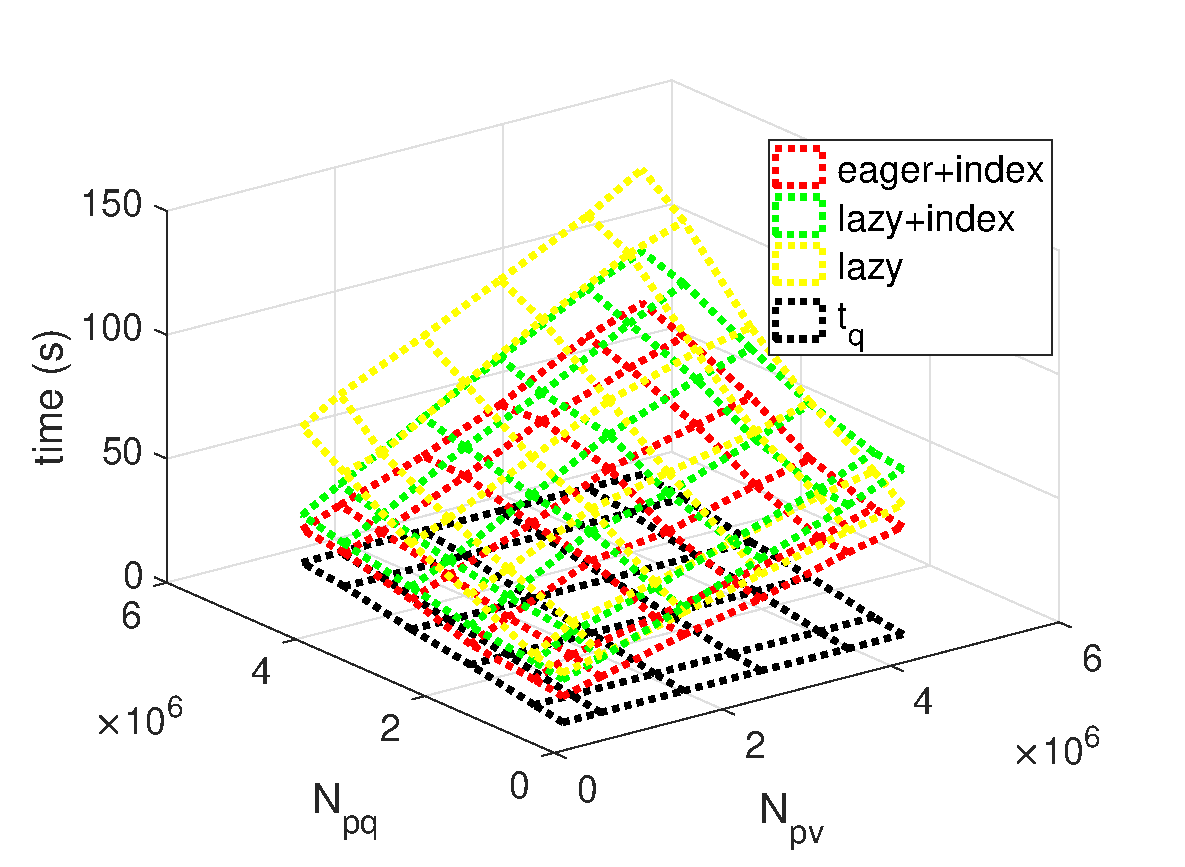
\includegraphics[height = 0.8\textwidth, width=1.2\textwidth]{Figures/synthetic_instance_size.eps}}
        \caption{$t_{total}$ with varied $N_{pq}$ and $N_{pv}$}     \label{fig:stress_test_instance_size}
    \end{subfigure}
    \hfill
    \begin{subfigure}{0.30\textwidth}
    \hspace*{-0.8cm}
        \raisebox{-\height}{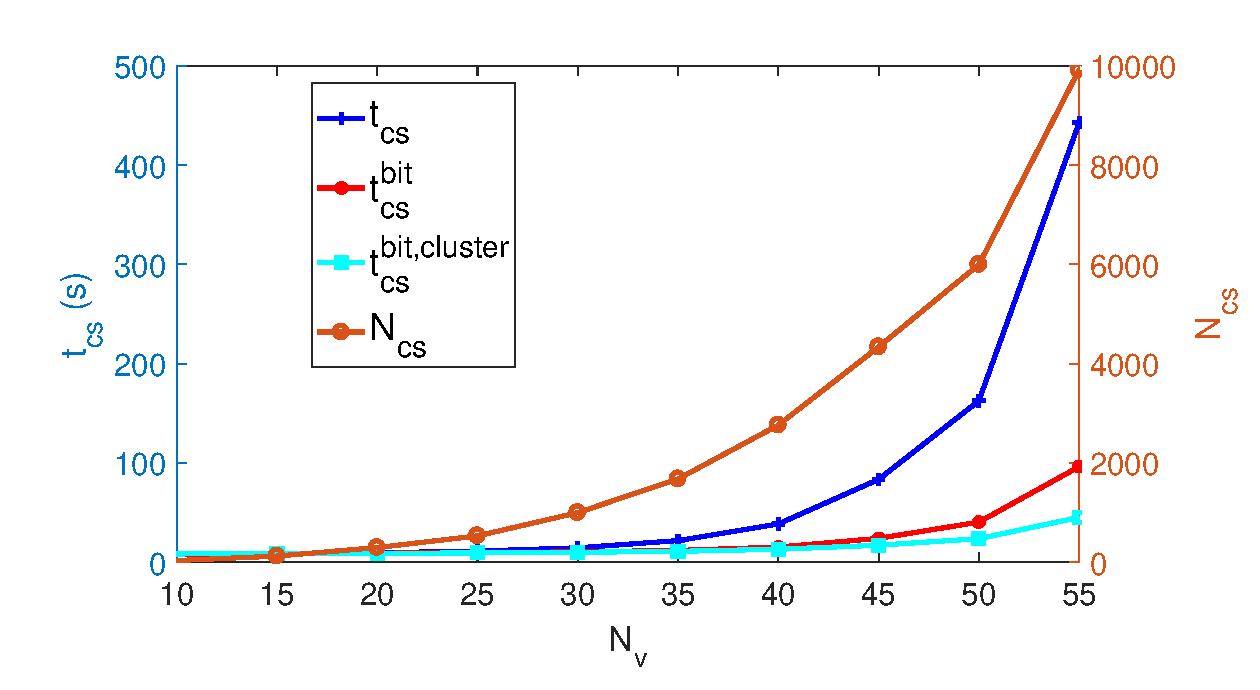
\includegraphics[height = 0.8\textwidth, width=1.2\textwidth]{Figures/synthetic_view_num.eps}}
        \caption{$t_{total}$ with varied $N_v$}
        \label{fig:stress_test_view_num}
    \end{subfigure}
    \hfill
    \begin{subfigure}{0.30\textwidth}
    \hspace*{-0.8cm}
        \raisebox{-\height}{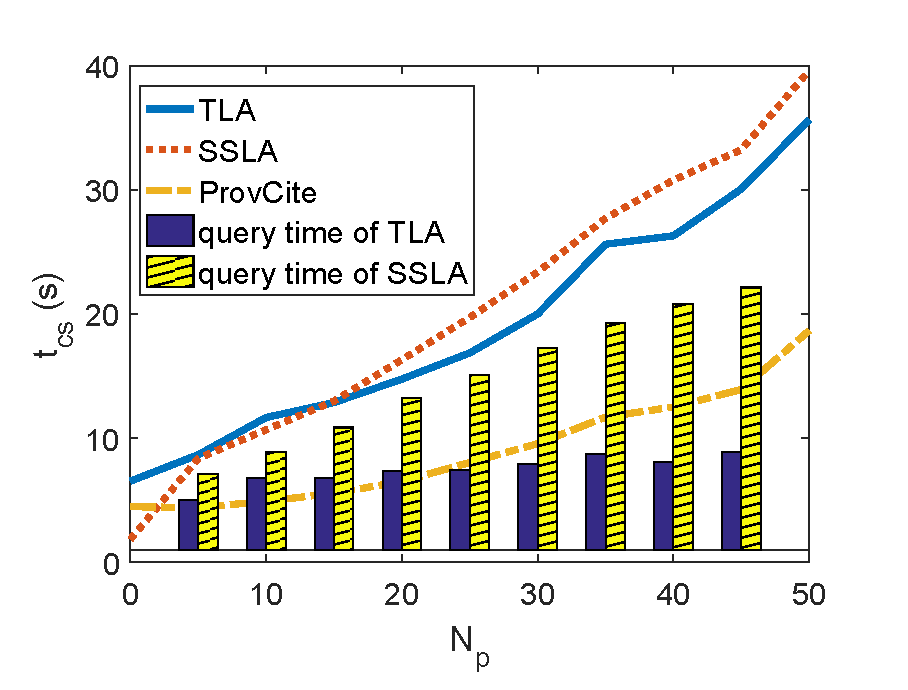
\includegraphics[height = 0.8\textwidth, width=1.2\textwidth]{Figures/synthetic_predicate_num.eps}}
        \caption{$t_{total}$ with varied $N_p$}
        \label{fig:stress_test_predicate_num_time}
    \end{subfigure}
    \caption{Experimental results for synthetic workloads}
\end{figure*}

Table \ref{Table: notation_summary} provides a summary of the notation mentioned in this subsection.% which will be used in the remainder of this section.

\subsection{Experimental results}
We now report on results from the synthetic and realistic workloads.

\subsubsection{Synthetic workloads} \label{sec: synthetic_exp}
We measured the impact of the provenance size of the query and view instances on time performance (Exp1), and the relative performance of \provalg\ and two implementations of \rba, TLA and SSLA,  while varying the view mapping number (Exp2) and the view predicate number (Exp3).

\textbf{Exp1.}  This experiment measures how the total execution time ($t_{total}$) is influenced by the total number of how-provenance monomials in the query instance ($N_{pq}$) as well as 
%the total number of how-provenance monomials 
in the view instance ($N_{pv}$). We randomly generate an aggregate query, and vary $N_{pq}$ by adding appropriate predicates. A fixed number of aggregate views are also generated such that there is exact one view mapping from each of them to the query and the total number of view mappings is fixed at 20.  In practice, the number of views that touch the query is usually far smaller than the total number of views, so 20 is a pretty large number. Both $N_{pq}$ and $N_{pv}$ are varied from 50K to 5M. The total time is measured for different ($N_{pq}$, $N_{pv}$) pairs under the {\em eager} and {\em lazy} strategy with the query provenance index, and the {\em lazy} strategy without the index. 

\textbf{Results.} 
The results are shown using 3D surfaces in Figure \ref{fig:stress_test_instance_size}, with the eager strategy with index, lazy strategy with index and pure lazy strategy shown in red, green and yellow respectively. The query time $t_q$ is also recorded in black. It shows that the query provenance index leads to about 1.0x-1.8x speed-ups in most cases by comparing lazy strategy with index and pure lazy strategy, while materializing view provenance results in about 1.1x-1.5x speed-ups by comparing eager strategy and lazy strategy with index. The combination of the index and eager strategy leads to up to 2x performance gains. The result also shows the {\em scalability} of our approach since it takes less than 2 mins to process a query instance with up to 5 million how-provenance monomials and 20 views with up to 5 million how-provenance monomials, which rarely happens in practice. \eat{We also observe that reasoning about valid view mappings is highly parallelizable, which means that further improvement can be achieved by implementing in distributed systems. }

% We also measured the extra space needed for the eager strategy, where the provenance of views is precomputed and stored in the database; it takes about 180 MB in the database to store the provenance for each view when the instance of the view includes up to 1 million how-provenance monomials. 

\textbf{Exp2.} The goal of this experiment is to compare the relative performance of \provalg, TLA and SSLA while varying the number of view mappings ($N_v$). Since TLA and SSLA cannot handle aggregate views, only conjunctive views are used. In this case, the provenance of views is not necessary; there is no difference between the eager and lazy strategy and the query provenance index is not useful. 
However, the two optimization strategies on covering set computation, i.e. applying bit arrays and clustering algorithms, are useful and are measured here.\eat{ We observe that \provalg\ have almost the same performance with TLA and SSLA no matter whether to use optimization or not and thus TLA and SSLA are not presented here.} The query is a fixed aggregate query with 1 million how-provenance monomials in its instance. $N_v$ is varied from 1 to 50 and there are no predicates or lambda variables for each individual view. 

\textbf{Results.}
The experimental results are presented in Figure \ref{fig:stress_test_view_num}, which shows the change of $t_{total}$ for ProvCide and the number of covering sets ($N_{cs}$) as the number of view mappings ($N_v$) increases, with and without using bit arrays and clustering algorithm. TLA and SSLA have almost the same performance as ProvCite, and are not shown. Figure \ref{fig:stress_test_view_num} shows that when $N_v$ is large, an exponential number of covering sets are generated, leading to bad performance (see blue line). Bit array computations and the use of clustering leads to about a 5x and 2x speed-up respectively; an order of magnitude performance gain is achieved by combining both.


\textbf{Exp3.} In this experiment, \provalg\ is compared with TLA and SSLA while varying the total number of predicates ($N_p$) in views. Similar to Exp2, the query is an aggregate query which can generate about 1 million tuples. The number of view mappings is fixed at 10 and there are initially no predicates. In each run, one more local predicate is added. As shown in \cite{wu2018data}, increasing $N_p$  significantly influences the query time and hence performance of TLA and SSLA since the query is extended to evaluate the view predicates. \eat{; 2) increasing the number of {\em reasoning groups} since we need to compute covering sets for each group and thus more {\em reasoning groups} in the query instance means more reasoning time. In theory, \provalg\ will also suffer from a large number of groups but will save on query time.}

\begin{table}
\centering
\small
\caption{Summary of datasets}
\vspace*{-0.2cm}
\begin{tabular}[!h]{|>{\centering\arraybackslash}p{2cm}|>{\centering\arraybackslash}p{1cm}|>{\centering\arraybackslash}p{2cm}|>{\centering\arraybackslash}p{2cm}|} \hline
Dataset name& \makecell{relation\\ \#} &average tuple \# per relation& tuple \# of largest relation \\ \hline
GENECODE&7&600k&2000k \\ \hline
Hetionet&38&60k&500k \\ \hline
DBLP-NSF&17&600k&6000k \\ \hline
\end{tabular}
\medskip
\label{Table: datasets_summary}
\caption{Notation used in the experiments}
\vspace*{-0.2cm}
\begin{tabular}[!h]{|c|>{\centering\arraybackslash}p{6cm}|} \hline
Notation & Meaning \\ \hline
$t_{cs}$&\makecell{total reasoning time to generate\\ the covering sets for all query tuples} \\ \hline
$t_{q}$&query time over the database \\ \hline
$t_{total}$&total execution time \\ \hline
$N_v$&total number of view mappings \\ \hline
$N_p$&\makecell{total number of predicates \\ under the view mappings} \\ \hline
$N_{pq}$&\makecell{total number of how-provenance\\ monomials in the query instance} \\ \hline
$N_{pv}$&\makecell{total number of how-provenance monomials \\in the view instance on average}\\ \hline
\end{tabular}
\medskip
\label{Table: notation_summary}
\caption{Experimental results on realistic datasets}
\vspace*{-0.2cm}
\begin{tabular}[!h]{|>{\centering\arraybackslash}p{0.75cm}|>{\centering\arraybackslash}p{1cm}|>{\centering\arraybackslash}p{0.85cm}|>{\centering\arraybackslash}p{0.85cm}|>{\centering\arraybackslash}p{0.7cm}|>{\centering\arraybackslash}p{0.25cm}|>{\centering\arraybackslash}p{0.25cm}|>{\centering\arraybackslash}p{0.6cm}|} \hline
Query& $t_{total}$ (s) (eager + index) & $t_{total}$ (s) (lazy + index)& $t_{total}$ (s) (lazy)& $N_{pq}$&$N_v$&$N_p$& $t_{q}$(s) \\ \hline
$q1$&11.05&12.93&11.89&1237k&1&0&5.09 \\ \hline
$q2$&1.75&2.06&3.26&203k&2&0&0.69 \\ \hline
$q3$&4.95&6.62&6.44&507k&2&0&2.92 \\ \hline
$q4$&5.90&6.49&6.33&416k&1&0&2.80\\ \hline
$q5$&4.65&5.10&4.81&243k&3&0&2.32 \\ \hline
\end{tabular}
\label{Table: realistic_performance}
\end{table}


\textbf{Results.} The results are shown in Figure \ref{fig:stress_test_predicate_num_time}\eat{, which matches the analysis above}. As the number of predicates increases, $t_{total}=t_{cs} + t_q$
increases slowly for \provalg. In contrast, TLA and SSLA are twice as slow as \provalg\ for large $N_p$. To understand the reason for this, the query time for TLA, SSLA and ProvCite is also presented in this figure, showing that the increasing query time becomes the major overhead for both TLA and SSLA. %, thus slowing down the computation.

{\bf Discussion.} The experiments reveal that all four metrics, $N_{pq}$ (the total number of how-provenance monomials in the query instance), $N_{pv}$ (the total number of how-provenance monomials in the view instance on average), $N_v$ (the total number of view mappings), and $N_p$ (the total number of predicates under the view mappings) can affect the total reasoning time $t_{cs}$. In extreme cases, where the value of the metric is very large, the performance of ProvCite is bad especially if implemented naively. However, the performance can be substantially improved using the bit array and clustering optimization strategies. We therefore expect ProvCite to have acceptable time performance for realistic workloads, where the extreme cases \eat{value of those metrics }rarely arise. 
% In the case of aggregate views where how-provenance is necessary, the  eager strategy beats the lazy strategy in terms of time.  The speedup is small (10\%-40\%), however, extra space is needed (up to 180 MB per view). So in practice, the choice between the eager or lazy strategy depends on whether speed or space is more important. In comparison to the previous approaches, TLA and SSLA, \provalg\ is not only more powerful in that it supports aggregate views but is also (surprisingly) frequently more efficient.  

\vspace*{-0.3cm}

\subsubsection{Realistic workloads}
\label{ssec: realistic}
The experimental results for realistic workloads are presented in Table \ref{Table: realistic_performance}, which includes the total execution time ($t_{total}$) for three cases (lazy, lazy + index and eager + index), as well as the metrics that can potentially affect the performance: the total number of how-provenance monomials in the query instance ($N_{pq}$), the total number of view mappings ($N_v$), the total number of predicates in the views under all the view mappings ($N_p$) and the time to query the provenance along with the instance. Except for $q1$, $t_{total}$ is less than 10 seconds for all queries. Although $N_{pq}$ is more than one million in $q1$, $t_{total}$ is only about 11-13 seconds for the three strategies, which is acceptable considering the large query instance. Note that the index does not always help since it may take significant time to build the index for query provenance (e.g. up to 3 seconds for $q1$) and its performance gain is not significant in the case of small number of view mappings.
% leads to weak effect of multiple scans over the entire query provenance.

However, as shown in Section \ref{sec: synthetic_exp}, the index provides  scalability especially in the extreme cases. We also list the query time over the provenance-enabled database in the last column, which indicates that the reasoning time ($t_{cs} = t_{total} - t_{q}$) is almost the same as $t_{q}$. Thus, while users are browsing the query result, the system can generate covering sets for all query tuples in the background, and instantly construct formatted citations upon tuple selection.

\eat{Comparing to time to simply generate query instance (See last column), $t_{cs}$ is still reasonable considering the large instance. When users are browsing the query result, the system can generate covering sets for all query tuple in the back-end, ready to construct formatted citations when users select tuples of interest.}

{\bf Discussion.} The experimental results show that reasonable time performance can be guaranteed in practice where none of the crucial metrics become too large.  Revisiting the experimental results for synthetic workloads, when the total number of how-provenance monomials in the query instance ($N_{pq}$) is about 1 million (as in $q1$), $t_{total}$ is about 1 min in the case of large $N_{pv}$ and $N_v$ values. However, since only one view mapping appears for $q1$, the time shown for $q1$ is  significantly smaller. \eat{ since the number of view mappings ($N_v$) is only 1, and the reasoning time relies on both $N_v$ and $N_{pq}$.} It also indicates that the number of view mappings should be small since views associate \textit{different parts} of the database with citations and thus only a small portion of them touch the query result\eat{the previous sentence is not very clear}. Performance is therefore acceptable in practise.